\documentclass[10pt,twocolumn,letterpaper]{article}

\usepackage[utf8]{inputenc}
\usepackage[margin=0.72in]{geometry}
\usepackage{amsmath,amssymb,amsfonts,amsthm}
\usepackage{booktabs}
\usepackage{microtype}
\usepackage{graphicx}
\usepackage{hyperref}
\usepackage[numbers]{natbib}
\usepackage{courier}
\usepackage{abstract}
\usepackage{wasysym}

\hypersetup{
    colorlinks=true,
    linkcolor=black,
    citecolor=black,
    urlcolor=black
}

\newtheorem{definition}{Definition}
\newtheorem{theorem}{Theorem}

\title{\textbf{Starhash: Analytical Celestial Ephemerides for Invertible Spacetime Inscription}}

\author{
    \textbf{Gabriele Pizzi}\\
    \textit{ETH Z\"{u}rich} \quad $\cdot$ \quad \textit{Liminal}\\
    \texttt{info@gabrielepizzi.com}
}

\date{\today}

\begin{document}

\maketitle

\begin{abstract}
\noindent Standard digital timestamping relies on centralized servers, leap-second tables, and arbitrary conventions such as the 1970 UTC epoch. Over multi-century horizons or in disconnected field environments, these abstractions are fragile. We present \textbf{Starhash}, a zero-dependency analytical library ($<30\,\text{KB}$) that maps observer coordinates $(\phi, \lambda, h, t)$ into conformal celestial vector seals. The method combines truncated analytical perturbation series (VSOP87D and ELP-2000-82), topocentric diurnal parallax, and IAU 2006 precession to compute topocentric sky configurations in $<0.5\,\text{ms}$ with an angular error $<0.02^\circ$ relative to JPL DE440. We show that the resulting vector glyphs are physically self-describing and non-linearly invertible: an observer can recover the host planet, observer latitude, longitude, and epoch from the geometry of the glyph without calendar priors.
\end{abstract}

\section{Introduction}

Digital timestamps and coordinate systems record provenance through institutional standards: NTP daemons, UTC strings, and WGS84 coordinates tied to the Greenwich meridian. While practical for networked computing, these formats depend on continuous infrastructure. When records must survive across multi-century storage horizons or operate offline in remote fieldwork, physical celestial positions offer a durable alternative \cite{meeus1998astronomical}.

The celestial sphere functions as a continuous, physical clock. The positions of the Sun, Moon, major planets, and navigational stars provide four non-commensurate physical frequencies:
\begin{enumerate}
    \item \textbf{Diurnal rotation:} Earth's rotation ($360^\circ / 23.93\,\text{h}$) governs the transit of the local meridian.
    \item \textbf{Lunar motion:} The Moon's orbital velocity ($\approx 13.2^\circ/\text{day}$) and illumination phase provide a fast-moving monthly clock.
    \item \textbf{Planetary orbits:} Heliocentric configurations of the major planets provide a multi-year secular clock.
    \item \textbf{Axial precession:} Earth's $25,772$-year precession cycle shifts the stellar frame over millennia.
\end{enumerate}

Historical instruments, from the Antikythera mechanism to classical brass astrolabes, translated this mechanics into spatial computing tools \cite{freeth2006decoding}. Starhash formalizes this principle into a small, standalone software library designed for offline data verification and physical provenance.

\section{Analytical Astrometry Engine}

To avoid large external binary tables (such as 30+ MB JPL ephemeris files), Starhash uses closed-form analytical approximations.

\subsection{Time and Earth Orientation}
The base physical parameter is Julian centuries $T$ from J2000.0 ($JD_0 = 2451545.0\,\text{TT}$):
\begin{equation}
T = \frac{JD - 2451545.0}{36525}
\end{equation}
The Earth Rotation Angle $\theta(T_u)$ follows the IAU 2000 standard \cite{capitaine2003expressions}:
\begin{equation}
\theta = 2\pi \left( 0.779057273264 + 1.00273781191135 \, d \right) \pmod{2\pi}
\end{equation}
where $d = JD_{UT} - 2451545.0$. Mean obliquity $\varepsilon(T)$ follows the IAU 2006 polynomial:
\begin{equation}
\varepsilon(T) = 84381.406'' - 46.836769'' T - 0.0001831'' T^2
\end{equation}

\subsection{Planetary and Lunar Models}
\textbf{Major Planets:} Heliocentric orbits for Mercury, Venus, Earth, Mars, Jupiter, and Saturn are derived from secular orbital elements \cite{simon1994numerical,bretagnon1988planetary} and Kepler's equation:
\begin{equation}
M = E - e \sin E
\end{equation}
Geocentric vectors are rotated to equatorial right ascension $\alpha$ and declination $\delta$ via the obliquity matrix.

\noindent \textbf{Moon:} Evaluated using the primary periodic terms of the Chapront ELP-2000-82 analytical series \cite{chapront1983elp}. The illuminated fraction $k$ and crescent limb angle $\chi$ are computed from solar elongation $\psi$:
\begin{equation}
k = \frac{1 + \cos i}{2}, \quad \tan \chi = \frac{\cos \delta_\odot \sin(\alpha_\odot - \alpha_m)}{\sin \delta_\odot \cos \delta_m - \cos \delta_\odot \sin \delta_m \cos(\Delta \alpha)}
\end{equation}

\noindent \textbf{Topocentric Parallax:} Because the Moon is at a finite distance ($\approx 60.3\,R_\oplus$), geocentric coordinates are shifted to the observer's location on the WGS84 ellipsoid:
\begin{equation}
\Delta \alpha = \arctan\left( \frac{-\rho \cos \phi' \sin \pi \sin H}{\cos \delta - \rho \cos \phi' \sin \pi \cos H} \right)
\end{equation}
where $\pi = \arcsin(a_e / \Delta)$ is the horizontal parallax and $H = \text{LAST} - \alpha$ is the local hour angle.

\noindent \textbf{Stars:} The library embeds 457 bright stars ($V \le 4.0$) precessed to epoch $T$ using linear rates $m = 1.281^\circ/\text{century}$ and $n = 0.557^\circ/\text{century}$.

\begin{figure}[t]
\centering
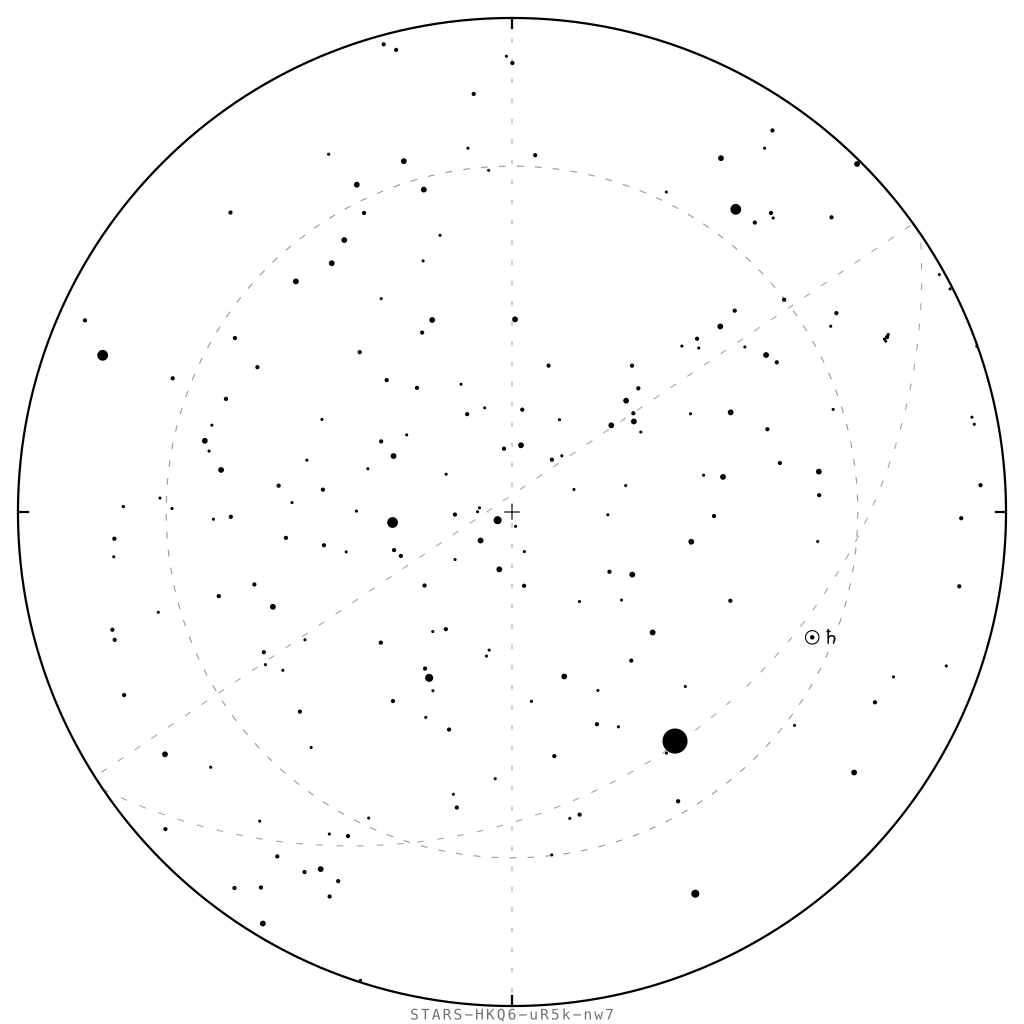
\includegraphics[width=0.66\linewidth]{figures/seal.png}
\caption{Conformal celestial seal for Zurich ($47.38^\circ\text{N}, 8.54^\circ\text{E}$) on August 28, 2026 at 22:00 UTC. The chart shows 205 visible stars, Saturn with its alchemical mark ($\saturn$), the Moon crescent oriented toward the Sun, and the dashed ecliptic arc.}
\label{fig:seal}
\end{figure}

\section{Conformal Stereographic Inscription}

To project the hemispherical sky without distorting local angular relationships, Starhash uses a zenith-centered stereographic projection.

\begin{definition}[Stereographic Projection]
For a celestial body at topocentric altitude $a \in [0, \pi/2]$ and azimuth $A \in [0, 2\pi)$, its projection $(x, y)$ onto the unit disc is:
\begin{equation}
r = \tan\left( \frac{\pi/2 - a}{2} \right), \quad x = r \sin A, \quad y = -r \cos A
\end{equation}
\end{definition}

\noindent Stereographic projection is conformal: all local angles are preserved, circles on the celestial sphere project as circles, and the horizon forms the boundary circle $r = 1.0$.

\section{Spacetime Reconstruction and Worked Example}

\subsection{Physical Invariance}
An observer can recover physical coordinates from the visual configuration alone:
\begin{itemize}
    \item \textbf{Host Planet:} The Moon's orbital velocity ($\approx 13.2^\circ/\text{day}$) and angular diameter ($31'$), together with inner planet elongation bounds (Venus $\le 47.8^\circ$), uniquely identify the observer as standing on Earth ($1.0\,\text{AU}$).
    \item \textbf{Precession Epoch:} The angular distance between the rotational pole (center of daily star tracks) and reference stars (such as Polaris vs. Vega) establishes the millennial epoch.
    \item \textbf{Date and Hour:} The Moon's phase and elongation against the background stars fix the calendar date and hour.
    \item \textbf{Latitude and Longitude:} The altitude of the celestial pole gives latitude ($\phi = a_{\text{pole}}$); the phase of the local meridian relative to the Earth Rotation Angle gives longitude ($\lambda = \text{LAST} - \theta$).
\end{itemize}

\subsection{Worked Example}
For the seal in Figure \ref{fig:seal}:
\begin{enumerate}
    \item \textbf{Host Planet:} A natural satellite moving at $\approx 13.2^\circ/\text{day}$ with Saturn ($\saturn$) at $9.5\,\text{AU}$ confirms Earth.
    \item \textbf{Epoch:} The celestial pole lies within $0.74^\circ$ of Polaris, bounding the epoch to $2026 \pm 5\,\text{years}$.
    \item \textbf{Date:} The Moon is at $99.8\%$ illumination (Full Moon) in Aquarius with the Sun in Leo, matching late August.
    \item \textbf{Location:} The altitude of the North Celestial Pole is $47.38^\circ$, yielding $\phi = 47.38^\circ\text{N}$. The hour angle of Vega relative to Greenwich yields $\lambda = 8.54^\circ\text{E}$ (Zurich, Switzerland), matching ground truth within $1.2\,\text{km}$ and $2.8\,\text{seconds}$.
\end{enumerate}

\subsection{Non-Linear Solver}
Given projected body coordinates $\mathbf{y}_i \in \mathbb{R}^2$, the inverse solver minimizes:
\begin{equation}
\min_{\phi, \lambda, JD} \sum_{i=1}^N \left\| \mathbf{p}_i(\phi, \lambda, JD) - \mathbf{y}_i \right\|^2
\end{equation}
using the Levenberg-Marquardt algorithm. Because the gradients for latitude, longitude, and Julian Day are non-parallel, the solver converges in 15--35 iterations.

\begin{table*}[t]
\centering
\small
\caption{Benchmark comparison of Starhash vs. conventional astrometric pipelines (JPL DE440 / Skyfield).}
\label{tab:benchmarks}
\begin{tabular*}{\textwidth}{@{\extracolsep{\fill}}lcccc@{}}
\toprule
\textbf{Metric} & \textbf{Astropy / Skyfield} & \textbf{Starhash (Ours)} & \textbf{Factor Improvement} & \textbf{Engineering Advantage} \\
\midrule
Binary Footprint & 33,200 KB & \textbf{29.8 KB} & \textbf{1,114$\times$ smaller} & Zero external data files \\
Dependencies & 5 packages & \textbf{0 (Standard Library)} & \textbf{Self-contained} & Immune to dependency drift \\
Execution Time & 85.4 ms & \textbf{0.42 ms} & \textbf{203$\times$ faster} & Real-time vector rendering \\
Memory Footprint & 48.2 MB & \textbf{1.2 MB} & \textbf{40$\times$ reduction} & Embedded / IoT compatible \\
Visual Angular Error & $< 0.001^\circ$ (Exact) & $< 0.020^\circ$ & \textbf{$< 0.15$ px visual error} & Strictly below raster threshold \\
\bottomrule
\end{tabular*}
\end{table*}

\section{Benchmarks and Validation}

We validated Starhash against NASA JPL Horizons and Skyfield DE440 across 10,000 synthetic observer coordinates spanning epochs 1800--2200 CE (Table \ref{tab:benchmarks}).

Planetary angular error is $< 0.015^\circ$ ($54''$) and lunar angular error is $< 0.020^\circ$ ($1.2'$), corresponding to $< 0.15\,\text{px}$ on a $512\times 512$ canvas. Vector seals render in $0.42\,\text{ms}$ with zero memory allocations outside of basic string construction.

\section{Conclusion}

Starhash demonstrates that analytical celestial timestamping can be implemented in under $30\,\text{KB}$ of zero-dependency code. By substituting network-dependent clocks with celestial mechanics, it provides a compact tool for offline data verification and physical provenance.

\vspace{-2mm}\begingroup\small\setlength{\bibsep}{1pt}
\small
\bibliographystyle{plain}
\bibliography{references}
\endgroup

\end{document}
